%
% Chapter 10
%

\chapter{Conclusion}
\label{conclusion}

In this dissertation, the search for the LFV decays of the SM Higgs boson into a muon and tau or an electron and tau has been presented. The search is performed with the full Run 2 data collected at the CMS experiment in 2016, 2017, and 2018 at a center-of-mass energy of 13~\TeV corresponding to an integrated luminosity of 137~\fb. The search found no evidence of the LFV decays of the Higgs boson, and corresponding exclusion upper limits have been placed on the branching fraction of Higgs boson into the \mutau and \etau final states.

The analysis is physics approved and is currently going through the CMS collaboration wide review process (as of January 2021) and is expected to be published in the Journal of High Energy Physics. The observed (median expected) upper limits on \BHmt is 0.15 (0.15)\,\% at 95\% CL and on \BHet is 0.22 (0.16)\,\% at 95\% CL. The limits on the branching fraction have been correspondingly translated into limits on the off-diagonal Yukawa coupling and are set to be $\sqrt{\Ymutau^{2}+\Ytaumu^{2}} < 1.11 \times 10^{-3}$ and $\sqrt{\Yetau^{2}+\Ytaue^{2}} < 1.35 \times 10^{-3}$.

These are the most stringent limits set in the LFV Higgs decays to date and constitute a significant improvement from the previous results. The previous analysis's expected limits are projected to the full Run 2 luminosity, which is accomplished by scaling the systematic uncertainties as inversely proportional to the square root of the luminosity. As can be seen in Figure~\ref{fig:projections}, the median expected limits from the current analysis are an improvement compared to the projections from the previous analysis. Several changes are performed compared to the previous search, and the various details have been explained in this dissertation in detail.

\begin{figure}[htbp!]
  \centering
  \subfigure[]{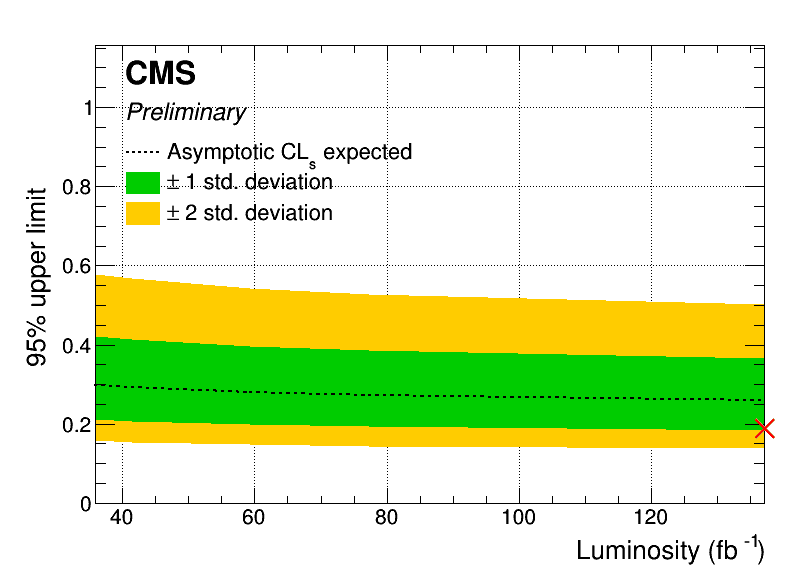
\includegraphics[width=0.4\textwidth]{plots/chapter10/MuTauh.png}}
  \hspace{0.5cm}
  \subfigure[]{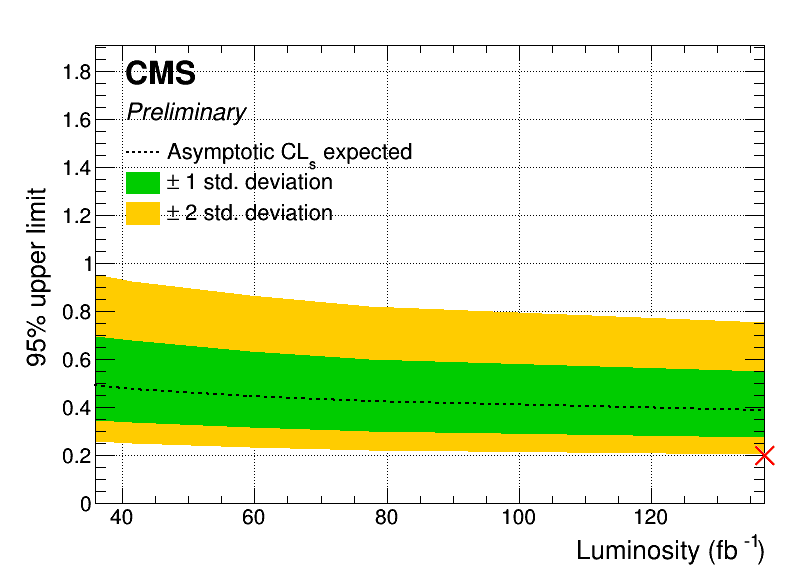
\includegraphics[width=0.4\textwidth]{plots/chapter10/ETauh.png}}\\
  \vspace{1cm}
  \subfigure[]{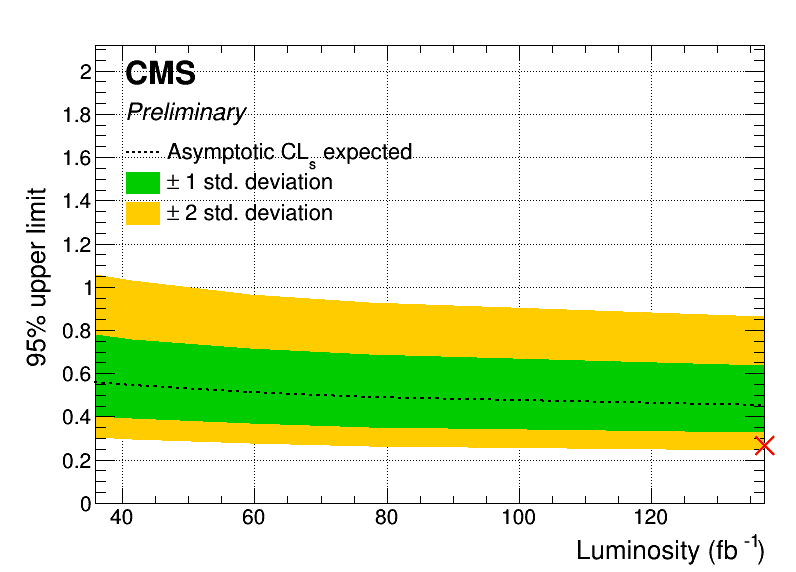
\includegraphics[width=0.4\textwidth]{plots/chapter10/MuTaue.png}}
  \hspace{0.5cm}
  \subfigure[]{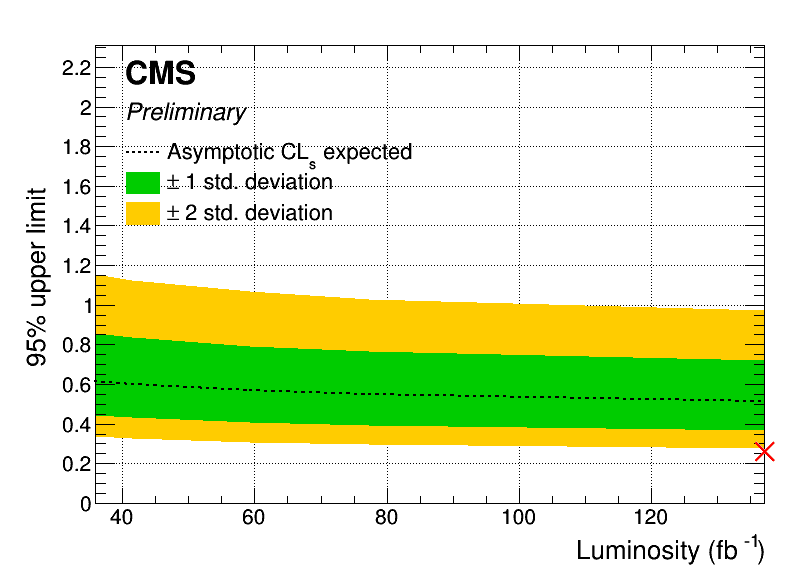
\includegraphics[width=0.4\textwidth]{plots/chapter10/ETaumu.png}}\\
  \vspace{1cm}
  \subfigure[]{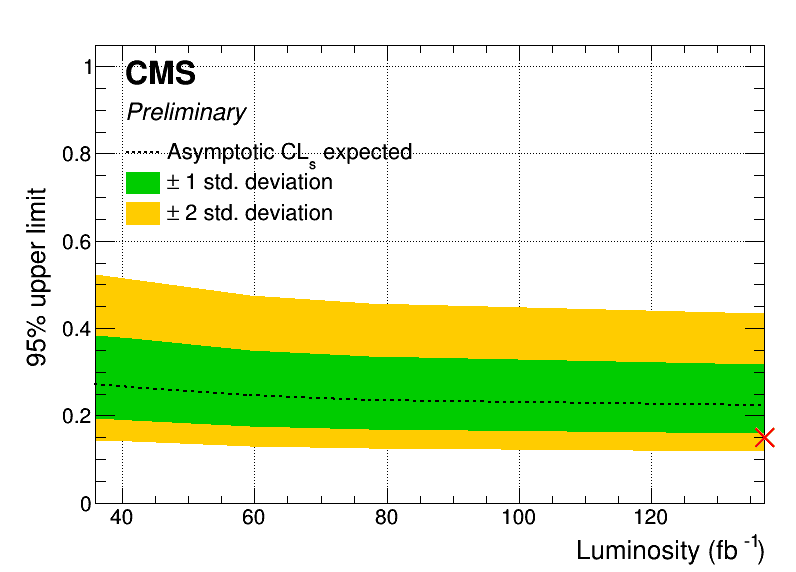
\includegraphics[width=0.4\textwidth]{plots/chapter10/MuTau.png}}
  \hspace{0.5cm}
  \subfigure[]{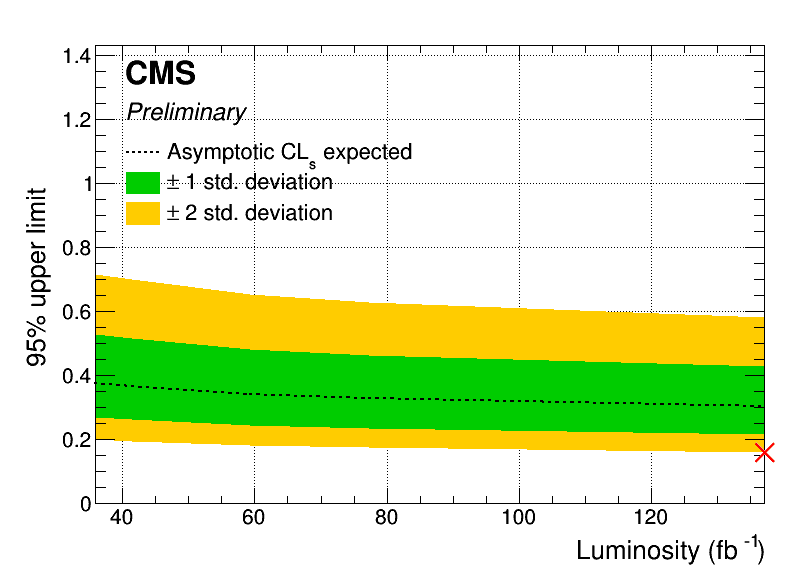
\includegraphics[width=0.4\textwidth]{plots/chapter10/ETau.png}}\\
  \caption{Expected limits from the previous analysis projected to the full Run 2 luminosity for (a) \muhad, (b) \ehad, (c) \mue, (d) \emu, (e) \mutau, and (f) \etau channels. The red cross represents the median expected limits obtained in the current analysis and are an improvement compared to the projections.}
  \label{fig:projections}
\end{figure}

In summary, using the DeepTau identification for the hadronically decaying tau leptons has significantly improved the sensitivity of the search in the hadronic channels. In the leptonic channels, the QCD background estimation technique has been updated. \Ztt background is estimated using the embedding technique for all channels and helps provide a good event description and better control over the systematic uncertainties. The misidentified lepton background in the hadronic channels has been modified. New shape systematics that weren't considered in the previous analysis are introduced to account for any residual discrepancies between the data and estimated backgrounds. All these improvements have compounded to set the most stringent limits on these branching fractions to date.

The LHC is expected to start taking data for Run 3 starting from the end of 2021, and currently, the expectation is that the center-of-mass energy will remain the same as for Run 2, i.e., 13~\TeV. We anticipate collecting approximately 150~\fb in Run 3, which will double the available dataset for Physics analysis. For the next iteration of this search, a new signal mass variable is proposed and is presented in the appendix~\ref{SVFit} (``Classic'' SVFit mass). From an initial study, this variable has been shown to improve the signal's mass resolution by approximately 20\%, which is a significant improvement. In appendix~\ref{fakefactor}, an improvement to the estimation of the misidentified lepton background in hadronic channels is presented, and it has the potential to improve the modeling and give a better handle over the systematic uncertainties that have a high impact on the median expected limits. Any future iteration of this search is highly recommended to use this mass variable for the signal mass hypothesis and the updated estimation of the misidentified lepton background in hadronic channels to improve the analysis's sensitivity.
